\section{Proposed Method}
\label{sec:method}


\begin{figure*}[t]
    \centering
    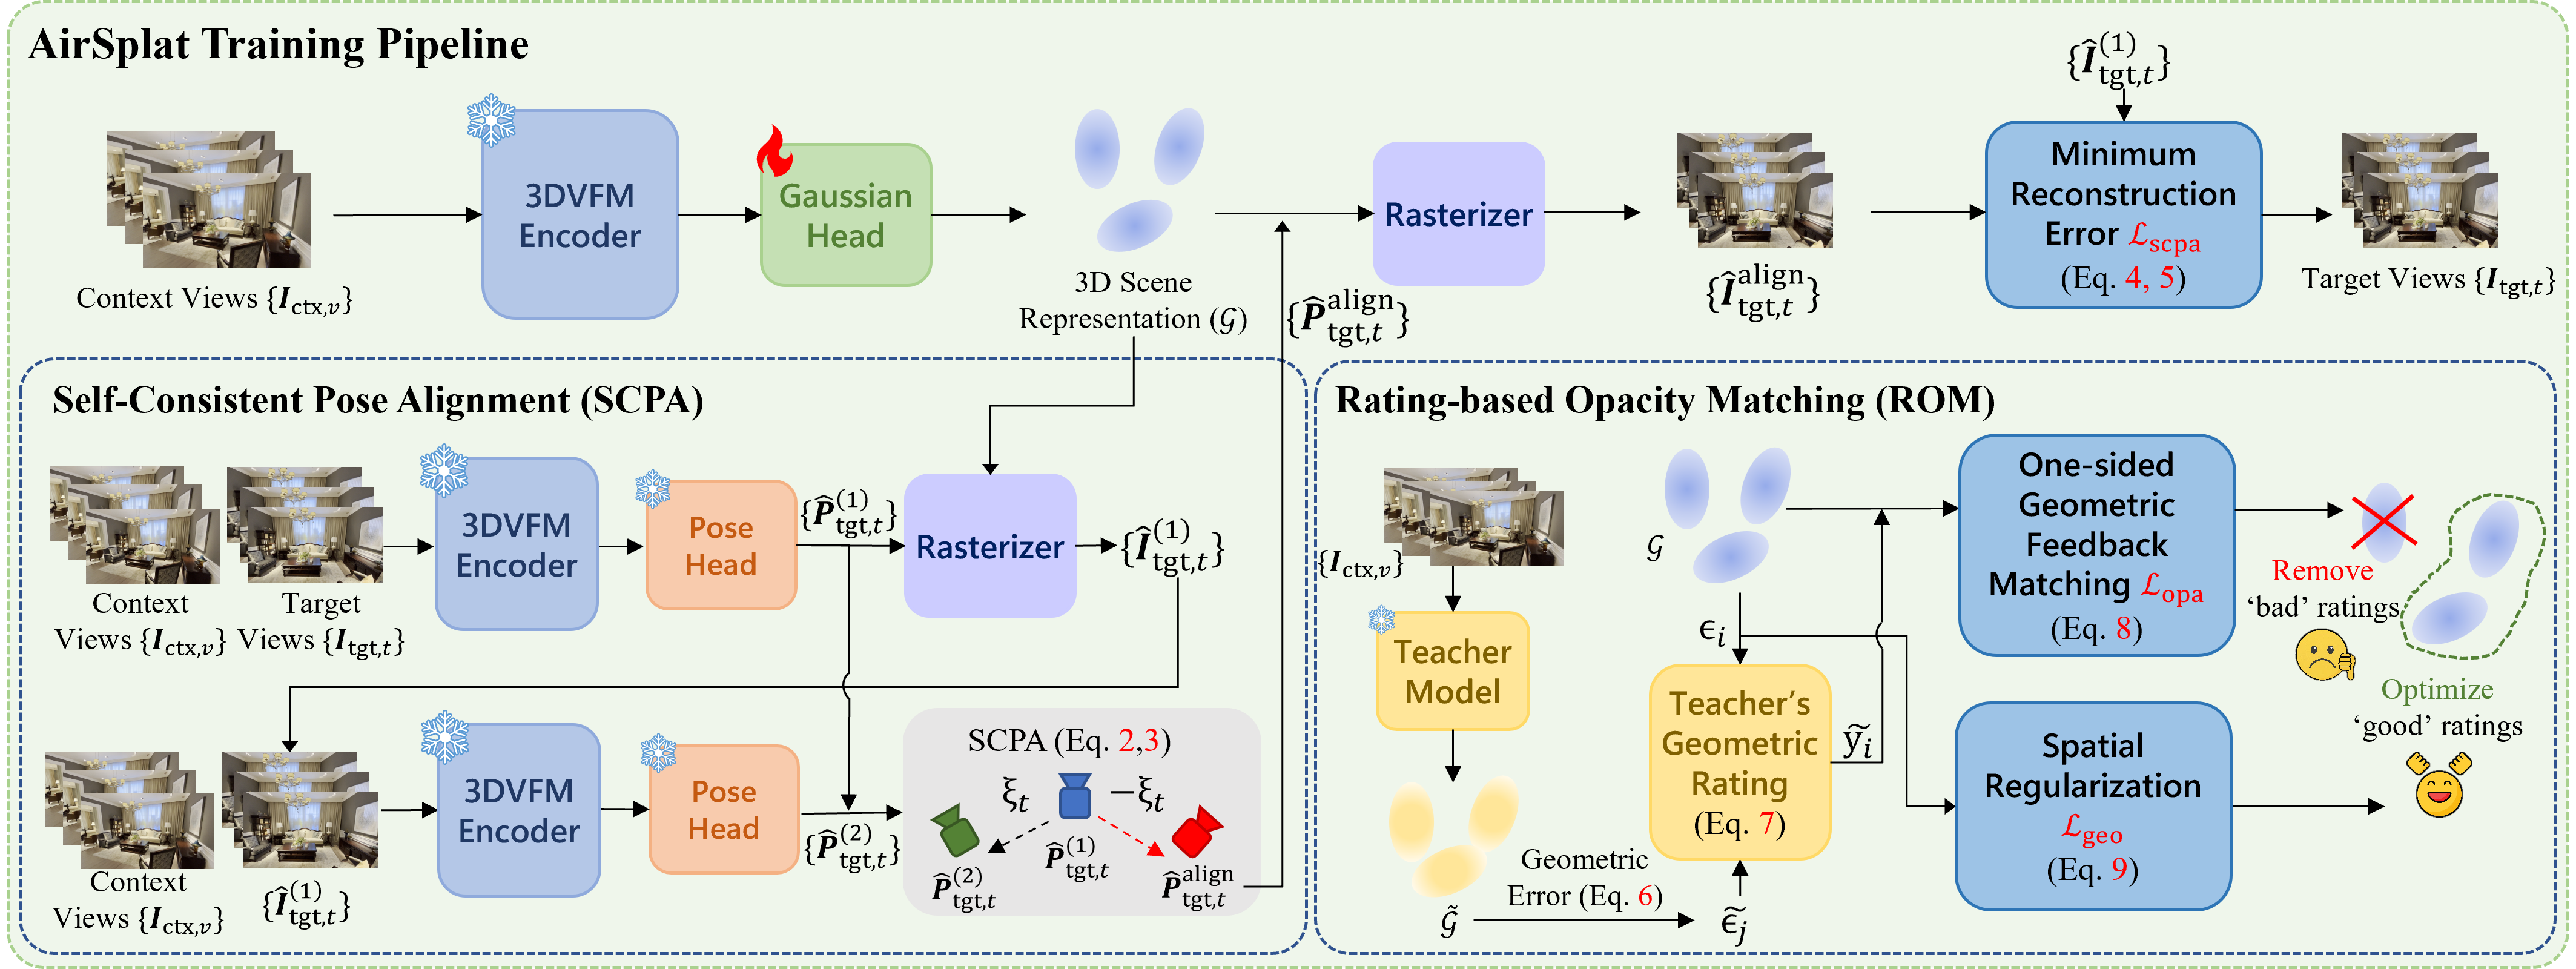
\includegraphics[width=\linewidth]{figures/main_architecture.png}
    \caption{Overview of our VFM-Splat.}
    \label{fig:main_architecture}
\end{figure*}

\subsection{Overview}

The objective of our framework is to synthesize high-fidelity novel views from sparse context images in a pose-free environment, leveraging the powerful geometric priors embedded in 3D Vision Foundation Models (3DVFMs). 
While 3DVFMs provide a strong initialization for geometry and camera poses, direct application for Novel View Synthesis (NVS) is hampered by two primary issues: local geometric inconsistencies across views and global coordinate misalignment during training.
To address these challenges, our method, introduces two core components:
\begin{enumerate}
\item \textbf{Self-Consistent Pose Alignment (SCPA)} addresses the pose-geometry discrepancy. We implement a training-time feedback loop that identifies the bias in initial pose predictions and back-extrapolates a corrected rendering pose. This ensures that the scene geometry is supervised by pixel-aligned photometric gradients.
\item \textbf{Rating-Based Opacity Alignment (RBOA)} focuses on local structural integrity and the removal of artifacts. Leveraging geometric ratings collected from a lightweight teacher model's feedbacks, we fine-tune the 3DVFM to align its predicted existence likelihood (opacity) with the teacher’s ratings. This mechanism effectively suppresses `undesirable' or geometrically inconsistent floaters through an asymmetric opacity compression margin, which ensures that only structurally sound primitives are preserved in the final radiance field.
\end{enumerate}



\subsection{Self-Consistent Pose Alignment}

\noindent \textbf{Pose Gap in Pose-free NVS Training.} 
In pose-free NVS training, the model is tasked with jointly inferring the 3D scene representation $\mathcal{G}$ and the target camera poses $\{\hat{\mathbf{P}}_{\text{tgt}}\}$. 
While the target poses are predicted using the joint features of both context and target views, i.e., $\mathbf{F}_{\text{joint}} = f_{\phi}(\{\mathcal{I}_{\text{ctx}}, \mathbf{I}_{\text{tgt}}\})$, the scene geometry $\mathcal{G}$ is conditioned strictly on the context views $\mathcal{I}_{\text{ctx}}$ to ensure generalizability during inference.
This asymmetric information flow creates a fundamental \textit{pose-geometry discrepancy} during training. 
Since the initial target pose $\hat{\mathbf{P}}_{\text{tgt}}$ is inferred from a predictive head $\psi_{\text{pose}}$ that has not yet seen the rendered 3D structure, it often lacks the strict geometric alignment required to reconstruct the ground-truth observation $\mathbf{I}_t^{\text{gt}}$.
When supervised by the standard reconstruction loss $\mathcal{L}_{\text{rec}}$ (Eq.~\ref{eq:rec_loss}), this misalignment propagates suboptimal gradients. Instead of refining the true 3D structure, the optimizer is forced to "blur" the Gaussians or introduce floating artifacts to compensate for the spatial shift caused by the pose error. 
Consequently, the model fails to capture sharp, consistent scene geometry, leading to degraded synthesis quality and temporal flickering.



\begin{figure*}[t]
    \centering
    \includegraphics[width=\linewidth]{figures/pose_corr_diff.png}
    \caption{Effect of our Self-Consistent Pose Alignment. Rendered target views using $\hat{\mathbf{P}}_{\text{tgt}}$ and $\hat{\mathbf{P}}_{\text{tgt}}^\text{align}$ and ground truth.}
    \label{fig:pose_corr_diff}
\end{figure*}


\noindent \textbf{Self-Consistent Pose Alignment} 
To bridge this gap, we propose \textit{Self-Consistent Pose Alignment} (SCPA), a training-time refinement mechanism that leverages the robust relative pose estimation capability of 3DVFMs.
Instead of directly supervising the noisy $\hat{\mathbf{P}}_{\text{tgt}}$, we introduce a self-correcting feedback loop. 
Given the predicted Gaussians $\mathcal{G}$ and the initial pose $\hat{\mathbf{P}}_{\text{tgt}}$, we render synthesized target images $\hat{\mathbf{I}}_t = \mathcal{R}(\mathcal{G}, \hat{\mathbf{P}}_{\text{tgt},t}), \quad \text{for } t=1, \dots, T.$.
We feed the rendered target images $\{\hat{\mathbf{I}}_t\}_{t=1}^T$ back into the 3DVFM along with the context views $\mathcal{I}_{\text{ctx}}$:
\begin{equation}
    {\hat{\mathbf{P}}_\text{ctx}^2, \hat{\mathbf{P}}_\text{tgt}^2} = \psi_{pose}(\mathbf{F}_\text{joint}^2), \quad \text{where } \mathbf{F}_\text{joint}^2 = f_{\phi}({\mathcal{I}_\text{ctx}, \{\hat{\mathbf{I}}_t\}_{t=1}^T}).
\end{equation}
The feedback pose $\hat{\mathbf{P}}_{\text{tgt}, t}^{2}$ effectively reveals the \textit{geometric bias} inherent in the current prediction pipeline. Specifically, if the model perceives the rendered content $\hat{\mathbf{I}}_t$ to be at $\hat{\mathbf{P}}_{\text{tgt}, t}^{2}$ despite being rendered at $\hat{\mathbf{P}}_{\text{tgt}, t}$, the transformation discrepancy $\Delta \mathbf{T}_t \in SE(3)$ represents the pose error that must be compensated:
\begin{equation}
    \Delta \mathbf{T}_t = \hat{\mathbf{P}}_{\text{tgt}, t}^{2} \cdot (\hat{\mathbf{P}}_{\text{tgt}, t})^{-1}.
\end{equation}

To align the rendering coordinate system with the target observation, we perform a first-order bias correction in the Lie algebra $se(3)$. By back-extrapolating the estimated bias, we derive the final aligned pose $\mathbf{P}_{\text{final}, t}$:
\begin{equation}
    \mathbf{P}_{\text{tgt}, t}^\text{align} = \Delta \mathbf{T}_t \cdot \hat{\mathbf{P}}_{\text{tgt}, t},
\end{equation}
where $\log(\cdot)$ and $\exp(\cdot)$ denote the logarithm and exponential maps for $SE(3)$, respectively.
Finally, we compute the reconstruction loss using the aligned pose $\mathbf{P}_{\text{tgt}, t}^\text{align}$ instead of the initial noisy estimate $\hat{\mathbf{P}}_{\text{tgt}}$. 
This ensures that the photometric gradients are backpropagated through a spatially consistent path, allowing the model to optimize for sharp and accurate scene geometry:
\begin{equation}
    \mathcal{L}_{\text{scpa}} = \sum_{t=1}^{T} \left( \| \mathcal{R}(\mathcal{G}, \mathbf{P}_{\text{tgt}, t}^\text{align}) - \mathbf{I}_t^{\text{gt}} \|_2^2 + \lambda_{s} \mathcal{L}_{\text{SSIM}} \right).
\end{equation}
Through this self-consistent loop, SCPA effectively decouples pose estimation errors from the geometry optimization, preventing the blurring artifacts commonly observed in pose-free NVS training.


\subsection{{Rating-Based Opacity Alignment (RBOA)}}

\noindent \textbf{Distilling Consistency from a Two-View Teacher.}
While our Self-Consistent Pose Alignment (SCPA) ensures global alignment, the scene representation $\mathcal{G}$ can still suffer from local geometric inconsistencies, such as "floaters" or artifacts that appear plausible from one view but vanish from others. 
To suppress these, we introduce Geometry-Guided Opacity Distillation (GGOD). 
We leverage a pre-trained two-view NVS model \cite{xu2025depthsplat} as a \textit{Teacher} to provide a reference for geometric consistency. 
The core idea is to evaluate the 3D-to-2D projection error of both the Teacher and the Student, then penalize the Student's opacity in regions where its inconsistency significantly exceeds the Teacher's baseline.

\noindent \textbf{Geometric Inconsistency Measurement.}
For a Gaussian mean $\mathbf{\mu}_v$ predicted from a center view $v$, we define its geometric inconsistency by projecting it onto an adjacent view $v'$ and measuring the distance to the corresponding sampled point. 
Let $\Pi_{v \to v'}(\cdot)$ be the projection-and-sampling operation using camera parameters $\{\mathbf{P}, \mathbf{K}\}$. 
The geometric error $\epsilon_v$ is formulated as:
\begin{equation}
    \epsilon_v = \frac{| \mathbf{\mu}_v - \Pi_{v \to v'}(\mathcal{G}) |_2}{\text{median}(\mathbf{D}_v) + \eta},
\end{equation}
where $\mathbf{D}_v$ is the depth map for normalization to ensure scale-invariance, and $\eta$ is a small constant for numerical stability. 
We compute this error for both the Student ($\epsilon_v^S$) and the Teacher ($\epsilon_v^T$).

\noindent \textbf{Excess Error and Opacity Ceiling.}
We define the \textbf{excess error} $\Delta \epsilon_v$ as the relative geometric deficiency of the Student compared to the Teacher:
\begin{equation}
    \Delta \epsilon_v = \max(0, \epsilon_v^S - \epsilon_v^T).
\end{equation}To effectively prune inconsistent Gaussians, we introduce a dynamic \textbf{opacity ceiling} $\bar{\alpha}_v$. 
This ceiling exponentially decays as the excess error increases, acting as a soft-mask for unfixable artifacts:
\begin{equation}
    \bar{\alpha}_v = \exp(-\gamma \cdot \Delta \epsilon_v),
\end{equation}
where $\gamma$ is a decay rate (e.g., $\gamma = 5.0$) determined by the sensitivity of the geometric inconsistency.


\noindent \textbf{Geometric Alignment Loss ($\mathcal{L}_{\text{geo}}$).} 
For Gaussians with resolvable discrepancies, we encourage the Student to minimize the excess error. 
To maintain stability against extreme outliers, we apply:
\begin{equation}
    \mathcal{L}_{\text{geo}} = \frac{1}{V} \sum_{v=1}^V \left( \text{min}(\Delta \epsilon_v, 2.0) \cdot \text{sg}[\alpha_v] \right),
\end{equation}
where where $\text{sg}[\cdot]$ is the stop-gradient operator that prevents backpropagation.

\noindent \textbf{Opacity Consistency Loss ($\mathcal{L}_{\text{opa}}$).} 
For Gaussians where the excess error is too high to resolve, we force the opacity to stay below the predicted ceiling:
\begin{equation}
    \mathcal{L}_{\text{opa}} = \frac{1}{V} \sum_{v=1}^V | \max(0, \alpha_v - \bar{\alpha}_v) |_2^2.
\end{equation}



\subsection{Loss Functions}
The overall optimization objective for training the Gaussian head $\psi_{gs}$ is designed to synergize global photometric alignment with local geometric distillation. 
While the 3DVFM $f_{\phi}$ provides high-level features, the loss functions ensure that these features are translated into a 3D representation that is both sharp and multi-view consistent. 
The total loss $\mathcal{L}_{\text{total}}$ is defined as:
\begin{equation}
    \mathcal{L}_{\text{total}} = \mathcal{L}_{\text{scpa}} + \lambda_\text{geo} \mathcal{L}_{\text{geo}} + \lambda_\text{opa} \mathcal{L}_{\text{opa}},
\end{equation}
where $\lambda_\text{geo}$ and $\lambda_\text{opa}$ are weighting hyperparameters that balance the reconstruction fidelity against the geometric priors.

% \subsection{Direct Geometric Preference Optimization (DGPO)}
% \label{sec:dgpo}

% \textbf{1. Probabilistic Formulation of Gaussian Existence:} 
% Recent works \cite{zhang20243dgsmcmc} have successfully framed the optimization of 3D Gaussian Splatting as sampling from an underlying probability distribution proportional to scene fidelity. We extend this probabilistic perspective to the feed-forward setting. We formulate our network as a generative policy $\pi_\theta(G | \mathcal{I})$ that predicts a set of 3D primitives $G = \{g_i\}_{i=1}^N$ given uncalibrated context views $\mathcal{I}$. 

% Crucially, rather than treating the opacity $\alpha_i \in [0,1]$ of primitive $g_i$ merely as a rendering alpha-blend value, we re-interpret it as the \textit{policy likelihood} of that primitive's geometric existence. An ideal policy should assign high existence probabilities ($\alpha \to 1$) to geometrically sound primitives and low probabilities ($\alpha \to 0$) to hallucinated artifacts or "floaters."

% \textbf{2. The Implicit Geometric Reward:}
% To align this policy without relying on costly Reinforcement Learning (RL) or computationally prohibitive dense multi-view rendering loops, we draw inspiration from Direct Preference Optimization (DPO) \cite{rafailov2023direct}. In DPO, a policy is directly aligned to maximize an implicit reward derived from human preferences. In our pose-free NVS setting, the "preference oracle" is the multi-view geometric consensus distilled from the 3D Vision Foundation Model (3DVFM).

% For a given predicted primitive $g_i$, we extract its spatial location from the network's prediction and cross-project it using the 3DVFM's distilled geometry. We define a continuous geometric penalty, the excess reprojection error $E_{geo}(g_i)$, as the discrepancy between the student's multi-view spatial variance and the teacher's geometric consensus:
% \begin{equation}
%     E_{geo}(g_i) = \max(0, \Delta_{\text{pred}}(g_i) - \Delta_{\text{teacher}}(g_i))
% \end{equation}
% The implicit reward for the primitive's existence is therefore inversely proportional to this error: $r(g_i) = -E_{geo}(g_i)$.



% \textbf{3. Deriving the Optimal Preference Policy:}
% Under the standard KL-constrained RLHF formulation \cite{rafailov2023direct}, the optimal policy $\pi^*$ that maximizes a reward $r(x)$ while anchoring to a reference behavior takes a closed-form Boltzmann distribution proportional to $\exp(\frac{1}{\beta} r(x))$. 

% Mapping this to our continuous opacity formulation, the optimal existence probability (the target opacity $\alpha_i^*$) for a primitive under the geometric reward strictly follows:
% \begin{equation}
%     \alpha_i^* = \exp\left( \frac{1}{\beta} r(g_i) \right) = \exp\left( -\frac{1}{\beta} \text{sg}\big(E_{geo}(g_i)\big) \right)
% \end{equation}
% where $\beta$ controls the temperature of the preference decay (empirically corresponding to a decay rate of $5.0$ in our implementation), and $\text{sg}(\cdot)$ is the stop-gradient operator. The stop-gradient ensures the network optimizes the policy likelihood rather than maliciously inflating the geometric error to trivially satisfy the loss.

% \textbf{4. The DGPO Loss Objective:}
% In discrete DPO, the network minimizes a binary cross-entropy over paired preference rankings. However, VFM-Splat operates on a continuous, unpaired reward signal for each generated token (Gaussian). Therefore, we formulate DGPO as a continuous, one-sided margin loss. 

% The optimal policy $\alpha_i^*$ represents the strict upper bound of geometric trust. If the network predicts an existence probability $\alpha_i$ that exceeds this geometric preference ceiling, the policy is penalized for overconfidence. The final Direct Geometric Preference Optimization loss is defined as:
% \begin{equation}
%     \mathcal{L}_{\text{DGPO}} = \frac{1}{N} \sum_{i=1}^{N} \Big( \max(0, \alpha_i - \alpha_i^*) \Big)^2
% \end{equation}
% By optimizing $\mathcal{L}_{\text{DGPO}}$, VFM-Splat dynamically suppresses the opacity of structurally unsound primitives in a single feed-forward pass, successfully aligning the 3D representation with foundation-level geometric priors without requiring iterative PPO or paired rejection sampling.
% GGOD distills knowledge from a pre-trained two-view teacher model using an optimization strategy. 
% We resolve spatial discrepancies through a geometric alignment loss while simultaneously suppressing fundamentally inconsistent floaters via a dynamic opacity ceiling. 

% This ceiling responds exponentially to the relative geometric error between the student and the teacher, effectively pruning artifacts that lack multi-view support.
% This ensures that the photometric gradients are backpropagated through a pixel-aligned path, preserving the sharpness of the scene geometry.